
\chapter{Introduction}
\label{chap:intro}
%%%%%%%%%%%%%%%%%%%%%%%%%%%%%%%%%%%%%%%%%%%%%%%%%%%%%%%%%%%%%%%%%%%%%%%
%%%%%%%%%%%%%%%%%%%%%%%%%%%%%%%%%%%%%%%%%%%%%%%%%%%%%%%%%%%%%%%%%%%%%%%
%%%%%Overview%%%%%%%%%%%%%%
%%%%%%%%%%%%%%%%%%%%%%%%%%%%%%%%%%%%%%%%%%%%%%%%%%%%%%%%%%%%%%%%%%%%%%%
%%%%%%%%%%%%%%%%%%%%%%%%%%%%%%%%%%%%%%%%%%%%%%%%%%%%%%%%%%%%%%%%%%%%%%%

\section{Prelude}
\label{sec: overview}
%what do we have inside galaxies:
% stuff we don't care about because they don't have a big contribution on the SED 1) planets; 2) black holes 3) dark matter
Inside every galaxy, there are millions of stars, planets, and black holes, as well as dust and gas.
They all affect each others' formation, evolution, and extinction.
There is also dark matter inside every galaxy, which, to the best of our knowledge, only has gravitational effects on the other components.
Nearly all the information we can obtain from galaxies other than our own comes from their light.
Since each observable phenomenon inside galaxies emits most of its energy in specific wavelengths, 
a plot of brightness/flux density of galaxies as a function of wavelength, call a spectral energy distribution (SED), is a useful tool to understand galaxies. 
Young and evolved stars, dust, and gas in the space between the stars are the most important contributors to the spectral energy distributions of galaxies.
Planets and black holes without an accretion disc, on the other hand, have a much lower intensity compared to the other aforementioned components, and therefore contribute less to the SED.
Therefore, with properly modeling observed features in SEDs we can extract information about the evolution of stars, dust, and gas inside galaxies.

%stars
Arguably, stars are the main component of normal galaxies.
They control the chemical composition and structure of galaxies by transforming gas into new stars and by transforming dead stars back into gas.
They are also central to the formation and evolution of planetary systems.
The energy provided by stars is necessary to create and maintain the life on planets. 
The study of the formation and evolution of the Sun, and more generally that of stars, helps us understand more about our origin and the future of our Solar System.
Furthermore, in order to completely understand the formation and evolution of galaxies from early universe to the current epoch, the knowledge of the formation and evolution of stars is necessary. 
As a result, the study of stellar formation and evolution has been a central topic in astronomy and astrophysics for decades.

%ISM 1)Gas 2)dust
%There could be a galaxy without stars (i.e. dark galaxies~\citep[][and references therein]{Cantalupo12}), but there will never be a galaxy without gas. %: this is a very strong statement. Some galaxies, like dwarf ellipticals, are pretty gas-free (at least now). So qualify this a bit. done
Among observable objects in galaxies, gas has a crucial role in formation and evolution of galaxies.
Gas and dust in galaxies can be found in the space between stars.
This space is called the interstellar medium (ISM), and is full of low density gaseous clouds with neutral or ionized atoms and/or molecules, and microscopic dust grains.
The gas and dust in the ISM are heated by interstellar radiation field and cool through a variety of line and continuum processes which usually depend on the local physical conditions. 
The effect of the ISM on stellar formation is undeniable; it provides the raw material for the formation of stars~\citep[e.g.][]{Kennicutt08,Bigiel08}.
Studying the interstellar medium is not only essential to understanding the formation of stars, but also it is necessary for interpretation of stellar evolution due to fact that stars release their material into ISM when they reach the end of their evolutionary track.

In a galaxy, like our own, star formation begins with the condensation of giant molecular clouds (GMCs, $\sim 10^7$ M$_{\odot}$) in the ISM due to gravitational instabilities. 
The denser regions within GMCs collapse under their own gravity (self-gravity) and create clumps.
Some of these clumps, which have a similar mass distribution to the stellar initial mass function (IMF), develop into self-gravitating cores.
Then these clumps continue to become denser and turn into protostars. 
Since the protostars have a higher mass than their surroundings, more gas from GMCs accretes onto protostars.
This procedure continues until hydrogen burning in centre of protostars starts (see~\cite{McKee07} for more detail). 

Metallicity, which is defined as the ratio of abundance of metals (any element heavier than hydrogen and helium) to the abundance of hydrogen, affects formation and evolution of stars indisputably.
\cite{Walch11} showed that in the case of large scale turbulence, the effect of metallicity on star formation is negligible, but if turbulence is decaying,  metallicity has a strong impact on stabilizing self-gravitating cores.
Metals also play an important role in heating, cooling, and ionizing processes in the ISM.
Since cooling is one of the main reasons for condensation of GMCs~\citep[e.g.][]{Maio07}, in low metallicity regions star formation may be suppressed. 
The amount of metals in stars affects their evolutionary tracks~\citep[e.g.][and references therein]{Maeder02}.
For instance, low metallicity stars tend to have lower mass loss via stellar winds than those with higher metallicity.
Observations show that massive low metallicity stars rotate faster.
Being more massive at the end of their evolutionary tracks gives massive low metallicity stars have a lower chance to explode and become a supernova.


%what does SED look like?
Our primary source of information about galaxies, specifically unresolved ones, is their spectral energy distributions. 
Broadly speaking, young and hot stars emit most of their light in ultraviolet (UV) wavelengths, evolved stellar populations show themselves in optical and near-infrared (NIR) emission, and gas and dust heated by stellar emission are bright in mid-infrared (MIR) or far-infrared (FIR) wavelengths.
Therefore, UV-to-IR SEDs contain valuable information about galaxies' stellar evolution and their ISM. 
Other wavelengths regimes in galaxy SEDs (e.g. X--ray, radio), that are dominated by processes such as active galactic nuclei, quasars, and supernovae shocks, are beyond the scope of this thesis.
The general shape of SEDs mirrors the morphological types of galaxies: starburst galaxies, which have high star formation rates (SFRs), emit the bulk of their energy in the UV, while the light of quiescent galaxies is dominated by optical and IR emission. 
Detailed information about the age of stellar populations and other properties of galaxies can be determined by modelling their SEDs.

 %how do you model it? %SED model CIGALE %Population synthesis ----> SFR, stellar mass 
The stellar population synthesis method, which sums stellar spectra to produce a composite spectrum, has been widely utilized since the 1970s~\citep[e.g.][]{Tinsley72,Searle73} to model SEDs of galaxies.
A thorough SED model must include stellar population models~\citep[e.g.][]{Bruzual93,Bruzual03,Maraston05}, stellar emission and dust attenuation~\citep[e.g.][]{Calzetti00,Dopita05}, dust grain emission such as from polycyclic aromatic hydrocarbons~\citep[PAHs; e.g.][and references therein]{Tielens08}, and IR emission from gas and dust~\citep[e.g.][]{Chary01,Dale02,Lagache03,Lagache04,Smith07a,Draine07}.
Many groups have modelled SEDs for different types of galaxies and created SED templates (for more information see the review of \cite{Walcher11} on fitting of SEDs and references therein).
Since the physical parameters of templates generated by the SED models are known, we can find properties of observed galaxies by fitting their SEDs (either by minizing $\chi^2$ or by Bayesian analysis), using the templates.
One example of an SED-fitting code is {\em CIGALE}: Code Investigating GALaxy Emission~\citep{Noll09}.
It combines SED models and uses Bayesian analysis to find the best-fit SED for observed data in the rest-frame UV-to-IR.
Some of the physical properties of galaxies must be assumed as model input find the best SED, and others are derived from SED-fitting results~\citep[see ][for more detail]{Walch08}.
For example, the best-fit SED has information regarding star formation history and stellar mass to light ratio.
By integrating star formation history over a specific time scale, SFR can be derived. %PB: please check: integrate SFH to get SFR, or integrate SFR to get SFH?
Knowing the stellar mass to light ratio, one can use a galaxy's observed luminosity to calculate its stellar mass.

The formation of stars in galaxies depends on many parameters including gas mass, stellar mass, metallicity, dust, the galaxy's morphology, and the location of the star forming region inside the galaxy.
In extragalactic astronomy, measuring the rate at which stars form is uncertain and relies upon theoretical models and observational data.
Studying star formation and its relation to other quantities in galaxies is the subject of ongoing research.
In this chapter, we present a review of observational methods of measuring the star formation rate and the main properties that affect measuring and scaling the SFR. A discussion of the ISM and its role in star formation is presented in $\S$~\ref{sec: ism_intro}. In $\S$~\ref{sec: sfr_intro} we discuss measuring the star formation rate, followed by a discussion of the measurement of the stellar mass in $\S$~\ref{sec: starmass_intro}. Current issues about star formation and its relation to other properties of a galaxy are discussed in $\S$~\ref{sec: pre_intro}. 
%% We or I?! %PB: use I


%%%%%%%%%%%%%%%%%%%%%%%%%%%%%%%%%%%%%%%%%%%%%%%%%%%%%%%%%%%%%%%%%%%%%%%
%%%%%%%%%%%%%%%%%%%%%%%%%%%%%%%%%%%%%%%%%%%%%%%%%%%%%%%%%%%%%%%%%%%%%%%
%%%%%ISM%%%%%%%%%%%%%%
%%%%%%%%%%%%%%%%%%%%%%%%%%%%%%%%%%%%%%%%%%%%%%%%%%%%%%%%%%%%%%%%%%%%%%%
%%%%%%%%%%%%%%%%%%%%%%%%%%%%%%%%%%%%%%%%%%%%%%%%%%%%%%%%%%%%%%%%%%%%%%%


\section{Components of the Interstellar Medium} 
\label{sec: ism_intro}
%how do we observe it
%what the observation tell us
% how do we measure the dust and gas
The interstellar medium in galaxies is a complex system with a wide range of structures, but these structures can be divided into two main components: gas and dust.
The gas in the ISM of galaxies is mostly made of hydrogen and helium, with 1 per cent heavier elements (metals), and can be in the form of clouds or diffuse (diffused?) regions.
Gas clouds include molecular clouds, cold neutral atomic hydrogen (\hi) or hot \hi~clouds, and diffuse gas can be either \hii~(ionized hydrogen) regions or a hot intercloud medium.
Dust is mostly comprised of silicates, and graphite grains can be seen in dark clouds or galactic cirrus.
Emission lines from atoms or ions (i.e \hii~regions) in a hot gas, lines from molecules in cold clouds, and 21~cm emission of \hi~are the main observational signatures of the gas in the ISM of galaxies.
Dust can be observed directly through far-infrared and sub-millimeter wavelength emission or indirectly through its extinction and attenuation effects (see Sec.~\ref{sec: extinction}).

Molecular clouds in the ISM are cold ($\sim10$ K) and dense ($ 50<n<500$ cm$^{-3}$); masses of molecular clouds range from a few to millions of solar masses~\citep{Bolato08}.
Density in the molecular clouds is not uniform. There are dense and colds clumps inside these clouds.
Since these clumps are ideal places to form stars, studying molecular clouds has an important role in understanding formation of stars.
However, H$_2$ molecules, the main component of molecular clouds, have no permanent electric dipole moment which makes them difficult to detect.
The second dominant component, helium, is a mono-atomic gas and has the same problem as hydrogen, but these clouds also contain heavier elements such as carbon monoxide, hydrogen cyanide, water, ammonia and more than tens of others.
Carbon monoxide (CO) molecules are the third-most abundant constituent of molecular clouds.
In fact, most of our knowledge from molecular clouds comes from observing line emission of CO molecules, which {\bf due to their heavy weight, they have very low energy rotational state} and can be excited in the temperature of molecular clouds.%%Sr: I'll add more detail here
Other heavier molecules have emission lines which are also detectable in the spectra of clouds (specially galactic ones), but observing CO emission is the most common way to study the properties of molecular clouds i.e. their mass (see Sec.~\ref{sec: ismmap} for more details).

The molecular clouds are surrounded by clouds of atomic gas~\citep{Kennicutt12}, which are easily traceable by 21-cm emission.
Hydrogen atoms in the ISM (excluding the regions close to hot stars, see below) are in their ground state. 
The electron and proton spins in the ground state can be parallel (i.e. both spin up) or anti-parallel (i.e. the proton's spin is up and the electron's spin is down or vice versa). 
The energy of the anti-parallel mode is slightly less than the parallel mode.
Since atoms always want to be in the state with lowest energy possible, electrons in the parallel mode have a tendency to flip to the anti-parallel mode. 
However, the energy difference between these two states is very small and it takes millions of years before the transition happens.
The large amount of hydrogen atoms compensates for the rarity of the transition and at any given time, there are enough hydrogen atoms to emit the 21-cm radiation. 
Observation of the \hi atoms is specifically necessary for understanding physical properties and dynamics of the ISM, which leads to understanding the star formation process~\citep{Walter08}.

\hii~regions are hot and low density regions that are mostly located in the disks of spiral galaxies.
High energy UV photons emitted by massive new born stars have sufficient energy to ionize their surrounding gas, and
~\halpha emission is the main observable feature of \hii~regions.
The temperature and density of these regions can be estimated by observing other recombination lines such as H$\beta$, and forbidden lines such as \sii, \oii, \oiii, and \nii. 
Forbidden lines are not called so because there is no chance of them occurring, but merely because their probability is much lower than the normal ``allowed'' transitions.
Optically bright \halpha emission from \hii~regions is correlated with number of new massive stars in regions, and can be used as a star formation tracer~\citep[e.g.][]{Kennicutt98b,Calzetti13}.
Studying \hii~regions provides valuable insight into star forming regions by providing information such as star formation rate, initial mass function (IMF), and distribution of ionizing stellar masses~\citep[][and references therein]{Azimlu11}.


Dust has an insignificant effect on the mass of the ISM, but it plays crucial roles in the ISM's evolution.
%The total gas mass of galaxies can be determined using optical depth in sub-mm waveband of dust emission. 
In spiral galaxies, dust grains are located in cold regions ($\sim$30~K) and have a power-law size distribution.
The source of energy for dust thermal emission is heating from stars, and the shape of the continuum depends on size of the grain.
Mid-infrared emission from dust grains is mainly dominated by PAHs heated by evolved stellar population~\cite{Smith07a} or recently formed intermediate-mass young stars~\cite{Peeters04}. 
Large grains that are either heated by light from star-forming regions or by the interstellar radiation field from total stellar population emit most of their light in far-infrared~\citep[e.g.][]{Calapa14, lu14}
Dust is the main source of extinction and reddening of starlight (see Sec.\ref{sec: extinction} for more information).

\subsection{Mapping the Interstellar Medium} 
\label{sec: ismmap}
Measuring the mass of gas in galaxies is a necessary step to knowing how much raw material is available for forming stars.
A map of the total gas mass in the ISM can be produced by direct observations of gas or using interstellar dust as a tracer. 
Neutral atomic and molecular hydrogen are the most common components of the ISM. 
Therefore, to produce a total gas mass map in galaxies, maps of these two components can be added together and multiplied by a constant factor to account for heavier elements (mostly helium) which cannot be observed directly. 
Another way to do the mapping is to assume that the ratio of total gas to dust is constant across the galaxy, and convert dust observations to a map of total gas mass.

\subsubsection{Direct Measurement of the Gas}

The surface density of gas in the ISM of galaxies can be measured by direct observation of the neutral and molecular hydrogen.
This method can be promising if observational data with resolved molecular and atomic clouds are available.
However, given the state of current technology, having high resolution images of clouds for most galaxies is not possible. 
This problem shows itself for distant galaxies more than nearby galaxies. 
As a result, using images of molecular and atomic gas clouds to measure surface density of gas in ISM is limited to the telescopes' resolution. 
 
%\subsubsection{Molecular Clouds}
%PB: some repetition from earlier subsection here. 
The carbon monoxide molecule has a weak permanent electric dipole moment and a ground rotational transition with low excitation energy. 
Given its low energy and critical density, CO can easily be excited even in cold molecular clouds.
Therefore, CO (usually the $J(1\rightarrow 0)$ rotational transition, observed at 2.6 mm) is used as a tracer of the mass of molecular clouds dominated by molecular hydrogen~\citep[e.g.][] {Sanders84}.
Higher rotational transitions of CO can be used as a tracer as well, but they are not as common as $J(1\rightarrow 0)$.

\cite{Young91} described the relationship between the CO luminosity of a cloud and its mass. The CO luminosity of a cloud is:
\begin{equation}
L_{CO} = D^2 \int I_{\rm CO} d\Omega, 
\end{equation}
%NOTE: Equations must be punctuated.%
where $D$ is the distance to the cloud and $I_{\mathrm CO}$ is the CO brightness temperature integrated over the line profile in K~km~s$^{-1}$.
It can be written as ${\int T_{\mathrm CO} dV}$ where $T_{\mathrm CO}$(k) is the peak brightness temperature in the CO line and $V$ is the line-width in km~s$^{-1}$.
For a uniform cloud with a radius $R$, the CO luminosity is given by:
 \begin{equation}
L_{\rm CO} = \pi R^2 T_{\rm CO} \Delta V.
\end{equation}

Giant molecular clouds are self-gravitating systems~\citep[e.g.][]{Efstathiou83,Blitz99}.
Thus, using the virial theorem leads to calculating the mass of the cloud: 
\begin{equation}
 \label{equ: vir}
 M_{cloud} = L_{\rm CO} \sqrt{\frac{4\rho}{3\pi G T_{\rm CO}}},
\end{equation}
where $\rho$ is the mass density of the cloud and $\sqrt{\frac{4\rho}{3\pi G T_{\rm CO}}}$ is called the conversion factor.
Equ.~\ref{equ: vir} shows that the total mass of molecular clouds and the CO luminosity of the cloud are directly related~\citep{Young91}. 
Since the dependence of $I_{\mathrm CO}$ on optical depth is negligible~\citep{Krumholz09}, total CO luminosity can be used to measure the total H$_2$ mass of galaxies.
The relation between CO emission and H$_2$ cloud mass is shown to be
\begin{equation}
N_{\rm H_2}/\rm cm^{-2} = X_{\rm CO} \times I_{\rm CO}/{\rm K km s}^{-1},
\end{equation}
where X$_{\rm CO}$ is the conversion factor (also known as the X-factor).
The X-factor is different for each galaxy and sometimes is even different in regions within a galaxy due to differences in properties such as metallicity.
Although assuming a constant conversion factor for galaxies like M82 and M31 can lead to accurate estimation of global molecular gas mass, in regions with low metallicity this assumption leads to uncertainties~\citep{Bolato13}. 
Various groups are working on observations of different types of galaxies to measure the X-factor for them~\citep{Wilson95, Bosselli02, Bolato13}.

\begin{figure}
\label{fig: mco}
\centering
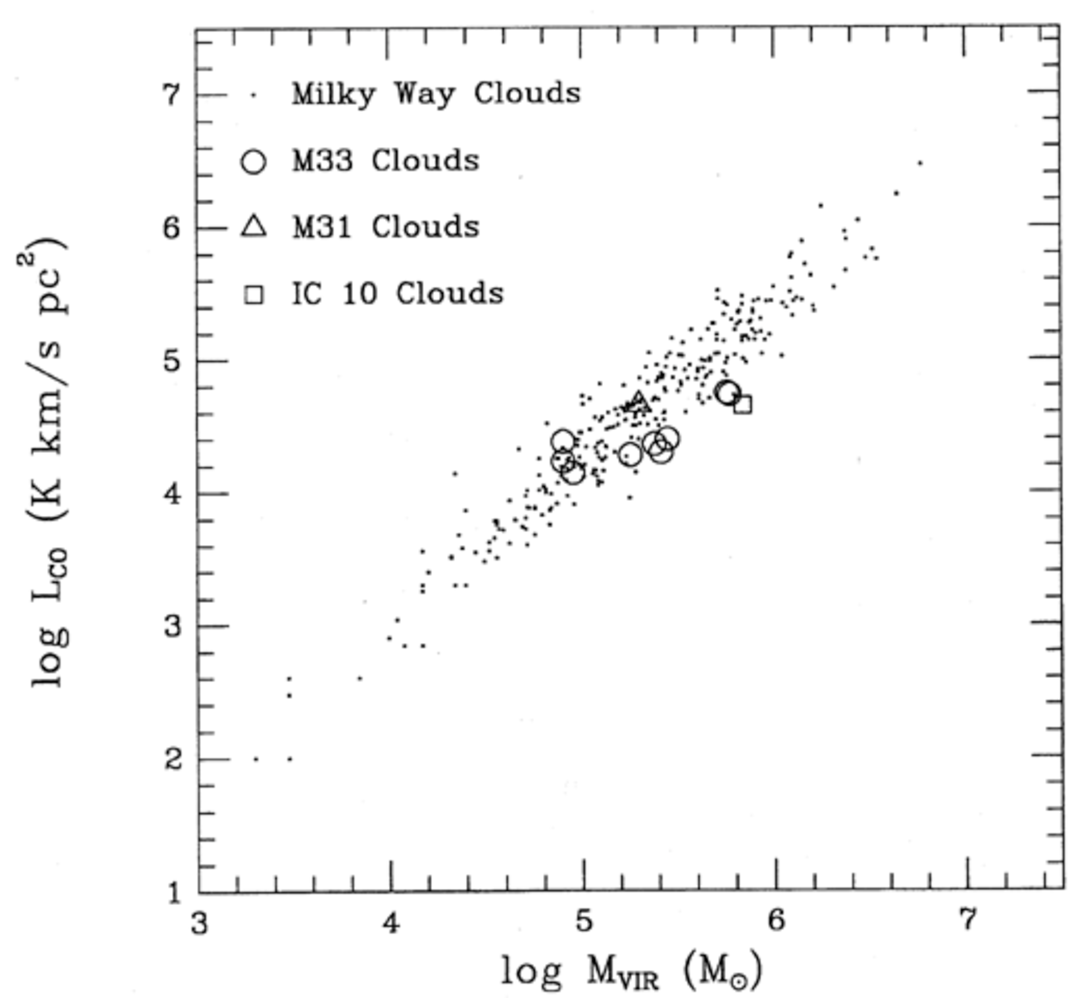
\includegraphics[width=16cm]{../image_intro/mvirial_lco.pdf}
\caption{Relation between the virial mass and CO luminosity for the Milky Way (dots), M33 (open circles), M31 (triangles), and IC~10 (squares) clouds. Virial masses are measured from selected high spatial resolution CO observations. The extragalactic molecular clouds are very similar to those in the Milky Way. Adapted from~\cite{Young91}.}
\end{figure}

In order to empirically determine the relation between H$_2$ masses and CO luminosities, many observational attempts have been made on both Galactic and extragalactic scales. 
One of the most significant studies in this regard was done by~\cite{Solomon87}, who studied this relation over more than 273 clouds inside the Milky Way and found a strong correlation between the virial mass of molecular clouds and CO luminosity. 
In Local Group galaxies, several groups have measured size, line width, and CO luminosity of molecular clouds and investigated the relation between  their virial masses and CO emission in environments other than the Milky Way. 
Pioneering works in measuring the extragalactic conversion factor were done for M31 and M32~\citep[e.g.,][]{Wilson89, Wilson90}. 
Fig.~\ref{fig: mco} shows the CO luminosity verses virial masses of molecular clouds in the Milky Way, M31, M33, and IC~10. 
The extragalactic molecular clouds are similar to those in the Milky Way. 
The conversion between the CO luminosity and H$_2$ masses is still a controversial topic~\citep[e.g.][]{Narayanan11, Bolato13, Sandstrom13}.
Problems regarding metallicity are not yet resolved and it is still not clear whether the conversion factor is global or local. 
Extragalactic investigations have been limited to nearby galaxies due to resolution and sensitivity of telescopes. 
To measure the clouds in distant galaxies, the spatial resolution of maps must be better than 40 pc, which is the typical size of a giant molecular cloud~\citep[e.g.][and refrences therein]{Young91,Bolato13}. 


%%%and now

Atomic gas in galaxies are dominated by \hi~atoms, which are relatively easy to observe in 21-cm.
Assuming optically thin lines for \hi~emission, the intensity of the 21-cm emission is proportional to the density of the atomic hydrogen, $N_{H {\sc I}}$~(cm$^{-3}$), along the line-of-sight.
\begin{equation}
N_{H {\sc I}}  \propto \int T_{\mathrm B} dV
\end{equation}
where $T_{\mathrm B}$ is the temperature brightness in Kelvins and dV is in Kms$^{-1}$, with the integral over the line profile. 
These properties make the 21-cm line a very useful tool to study gas in the ISM and trace the large-scale distribution of galaxies in the universe (\hi is detectable in most spiral galaxies and some elliptical galaxies).
Although the 21-cm emission is the most reliable technique to map the ISM, the linear relationship between the intensity and the column density of the gas breaks down when the gas is optically thick~\citep{Braun09}. 

\subsubsection{Dust Emission as a Tracer of Gas} 

Studying the gas clouds in the ISM of distant galaxies by using direct methods is almost impossible and not practical, due to low spatial resolution of data.
\cite{Hildebran83} was the first to suggest that one way to estimate the mass of the gas in the ISM might be from the optical depth of the sub-mm continuum emission from the dust; continuum dust emission is generally optically thin. 
The Herschel Space Telescope \cite{Pilbratt10} has measured the continuum dust emission from hundreds of galaxies\citep{Eales10, Oliver12}. 
This amount of observational data provides a unique opportunity to study the ISM of galaxies using dust emission. 
The observed FIR flux has almost no dependency on distance, thus, one of the advantages of using the dust emission as a tracer of the gas mass is that unlike the direct method, high spatial resolution is not necessary. 
The other important advantage is that this method solves the newly-found problem of ``dark gas" in galaxies. 
Dark gas is a significant fraction of gas in galaxies which can be traced by neither the 21-cm emission nor the CO emission~\citep{Abdo10}. 
As such, it is very difficult to detect with telescopes, but an accurate gas to dust ratio can lead to an accurate estimate of dark gas mass in galaxies. 

There are disadvantages in using the gas to dust ratio to trace gas in the ISM.
In order to use the dust as a tracer of the gas mass, first a relationship between the optical depth and the mass of the dust and then a relationship between the mass of the dust and the mass of the gas must be derived.
\cite{Draine03} pointed out that the former approach is uncertain because of the uncertainly in the radiative efficiency of dust grains. 
Measuring the gas to dust ratio in galaxies are not accurate either~\citep{Hildebran83}, which means that there are problems in both steps. 
In addition, the dust method has two major practical problems: firstly, to apply this method, knowing the temperature of the dust is necessary. 
To solve this problem, measurement of the continuum emission at far-infrared wavelengths long enough to cover the peak of the emission must be very accurate~\citep{Ealas12}. 
The other problem is that there is evidence that the gas to dust ratio depends on the metallicity of the gas~\citep{Lisenfeld98, Draine07}, but even in direct methods the dependence on metallicity must be solved. 
This (MH: This method? what does this refer to?) method is the best alternative for measuring the total gas in galaxies, that there is no observation of CO or \hi~emission. 

\subsection{The ISM and starlight: extinction and attenuation}
\label{sec: extinction}
Dust in ISM affects stellar emission by attenuating, scattering or absorption.
Attenuation refers to the effects of dust with embedded light sources distributed throughout. (MH Very unclear sentence)
The dust itself can be clumpy or smooth. 
Effect of dust clouds with embedded light sources on distribution of the light is called attenuation. (MH I though you defined attenuation two sentences ago, albeit unclearly.)
The dust cloud could have any distribution and be clumpy or smooth. (MH Deja vu)
Since both light source and dust have extended distribution, the relative location of the dust and light source affect the net absorbed and scattered light.
The other parameters that are important for the scattering and absorption is the relative position of dust and observer.
When the dust is in the line of sight, attenuation will make the emerging light dimmer~\citep[e.g.][and references therein]{Calzetti13}.
This is the typical occurring situation when studying galaxies or extended regions within galaxies.

Extinction happens when there is a combination of both absorption and scattering of radiation by dust.
This effect grows inversely with the wavelength.
Extinction can be defined as a reduction of the original intensity caused by dust:
\begin{equation}
\label{equ: extinction}
{\mathrm I}(\lambda) = {\mathrm I}_0(\lambda)exp[-\tau_{\lambda}],
\end{equation}
where I$(\lambda)$ is observed intensity in wavelength $\lambda$, I$_0(\lambda)$ is intensity of light before passing through dust, and $\tau_{\lambda}$ is extinction in $\lambda$.
The extinction also depends on size of grains and extinction cross section.
For measuring SFR using various wavebands, decreasing of the intensity of radiation must be calculated and corrected for each wavelength; otherwise, there will be an underestimation of SFR. 

%%%%%%%%%%%%%%%%%%%%%%%%%%%%%%%%%%%%%%%%%%%%%%%%%%%%%%%%%%%%%%%%%%%%%%%
%%%%%%%%%%%%%%%%%%%%%%%%%%%%%%%%%%%%%%%%%%%%%%%%%%%%%%%%%%%%%%%%%%%%%%%
%%%%%SFR%%%%%%%%%%%%%%
%%%%%%%%%%%%%%%%%%%%%%%%%%%%%%%%%%%%%%%%%%%%%%%%%%%%%%%%%%%%%%%%%%%%%%%
%%%%%%%%%%%%%%%%%%%%%%%%%%%%%%%%%%%%%%%%%%%%%%%%%%%%%%%%%%%%%%%%%%%%%%%

\section{Measuring the star formation rate in galaxies} 
\label{sec: sfr_intro}
Understanding the formation of stars leads to better understanding of galaxies' formation and evolution. 
Characterisation of the star formation processes such as star formation rate (SFR) and the stellar initial mass function (IMF) is necessary in examining galaxies' structure formation~\citep{McKee07}. 
Measuring the SFR is not trivial and depends on a galaxy's morphology, metallicity, IMF, observational spatial resolution, and other properties. 
There is a large number of review papers on how stars form and how their formation is traced. 
From a theoretical perspective, one can refer to the classic picture of the theory of star formation as reviewed by \cite{Shu87} and more recently by~\citep{McKee07}. 
From an observational standpoint, star formation is discussed by \cite[][and references therein]{Kennicutt98b, Kewley02, Calzetti13, Boquien10, Kennicutt12}.

In principle, emission from new stars can be traced by ultraviolet, visible light, near-IR and radio wavelengths, hydrogen recombination lines, forbidden metal lines, and also in the sub-mm range by using the Bremsstrahlung emission. 
Some of this emission is directly from stars, e.g.\ UV emission, and some is from ISM components that absorb and re-emit light from young stars, e.g.\ far-infrared emission.
Techniques to calibrate emission from newly-born stars, preferably hot and massive ones, to the rate at which stars are being formed have been the subject of many studies~\citep[e.g.][]{Calzetti07, Kennicutt11, Hao11,Bigiel08} 
Peak of emission of young, hot, and massive stars is in UV wavelength, which makes them an ideal tracer of the current SFR.
One of the main assumptions in using the luminosity of massive stars is that the SFR has remained largely constant during the timescale probed by the specific wavelength which is being used as the tracer. 
By knowing the IMF, the number of massive stars can be used to extrapolate the total number of stars formed in a given star-forming region.
To have a reliable SFR indicator, the stellar IMF must be fully sampled to have at least one star in all mass bins (for more detail see Sec.~\ref{sec: imf}).
In general each tracer has some systematic errors, and one should decide which tracer is more accurate for a given system. 

\subsection{Stellar Initial Mass Function}
\label{sec: imf}
Stellar mass determines the important properties of a star, such as luminosity, lifetime and its evolutionary path. 
One of the most fundamental and difficult questions that a complete theory of star formation must answer is what is the stellar initial mass distribution of a star forming region.
Since most SFR calibrations use emission from stars in a specific mass range, it is necessary to know the stellar IMF to extrapolate to the full stellar population.
\cite{Salpeter55} empirically derived the stellar IMF from the observed stellar luminosity function of the Solar neighbourhood~\citep{Shu87}. 
He introduced a power-law IMF $\Phi$  in the form:
\begin{equation}
\label{equ: salp}
\Phi (\log M) = dN / d \log M \propto M^{-\gamma }
\end{equation} 
where $M$ is the stellar mass, $\gamma$ is a power index, and $N$ is the number of stars in the logarithmic mass range of $\log M + d\log M$.

In the late 70s, it was recognised that the assumption of a the single power-law IMF over all stellar masses is not correct and might overestimate the number of low-mass stars~\citep{Kroupa93, Bastin10}. 
Since then, many groups have studied the stellar IMF and found different power-law relations (Fig.~\ref{fig: imf} ). 
Most SFR calibrations have the same assumption that the stellar IMF is constant across all environments and adopt it from the standard stellar IMF introduced by\cite{Kroupa01}:
\begin{equation}
\begin{split}
    \Phi (\log M) & \propto M^{-2.3}    \quad    (0.1 \le M(M{\odot}) \le 0.5)\\                  
           & \propto M^{-3.3}    \quad    (0.5 \le M(M{\odot}) \le 100)
\end{split}
\end{equation}
Although the Salpeter IMF produces more low-mass stars than the Kroupa IMF, they produce almost the same number of high-mass stars. 
Therefore, the SFR calibrations, which mostly trace massive stars in galaxies, based on the Kroupa IMF can be converted to the Salpeter IMF by multiplying the calibration constant by 0.67~\citep{Madau14}.
In a more recent study,~\cite{Weisz15} used data from the Panchromatic Hubble Andromeda Treasury program~\citep[PHAT][]{Dalcanton12} and showed that for nearby galaxies both Kroupa and Salpeter stellar IMFs overestimate the number of stars with masses greater than 8M$_\odot$.
\cite{Bastin10} reviewed the stellar IMF as derived from many observational results and showed that the stellar IMF is constant and universal, though there are uncertainties in different mass bins especially at the high-mass end. 

\begin{figure}
\label{fig: imf}
\centering
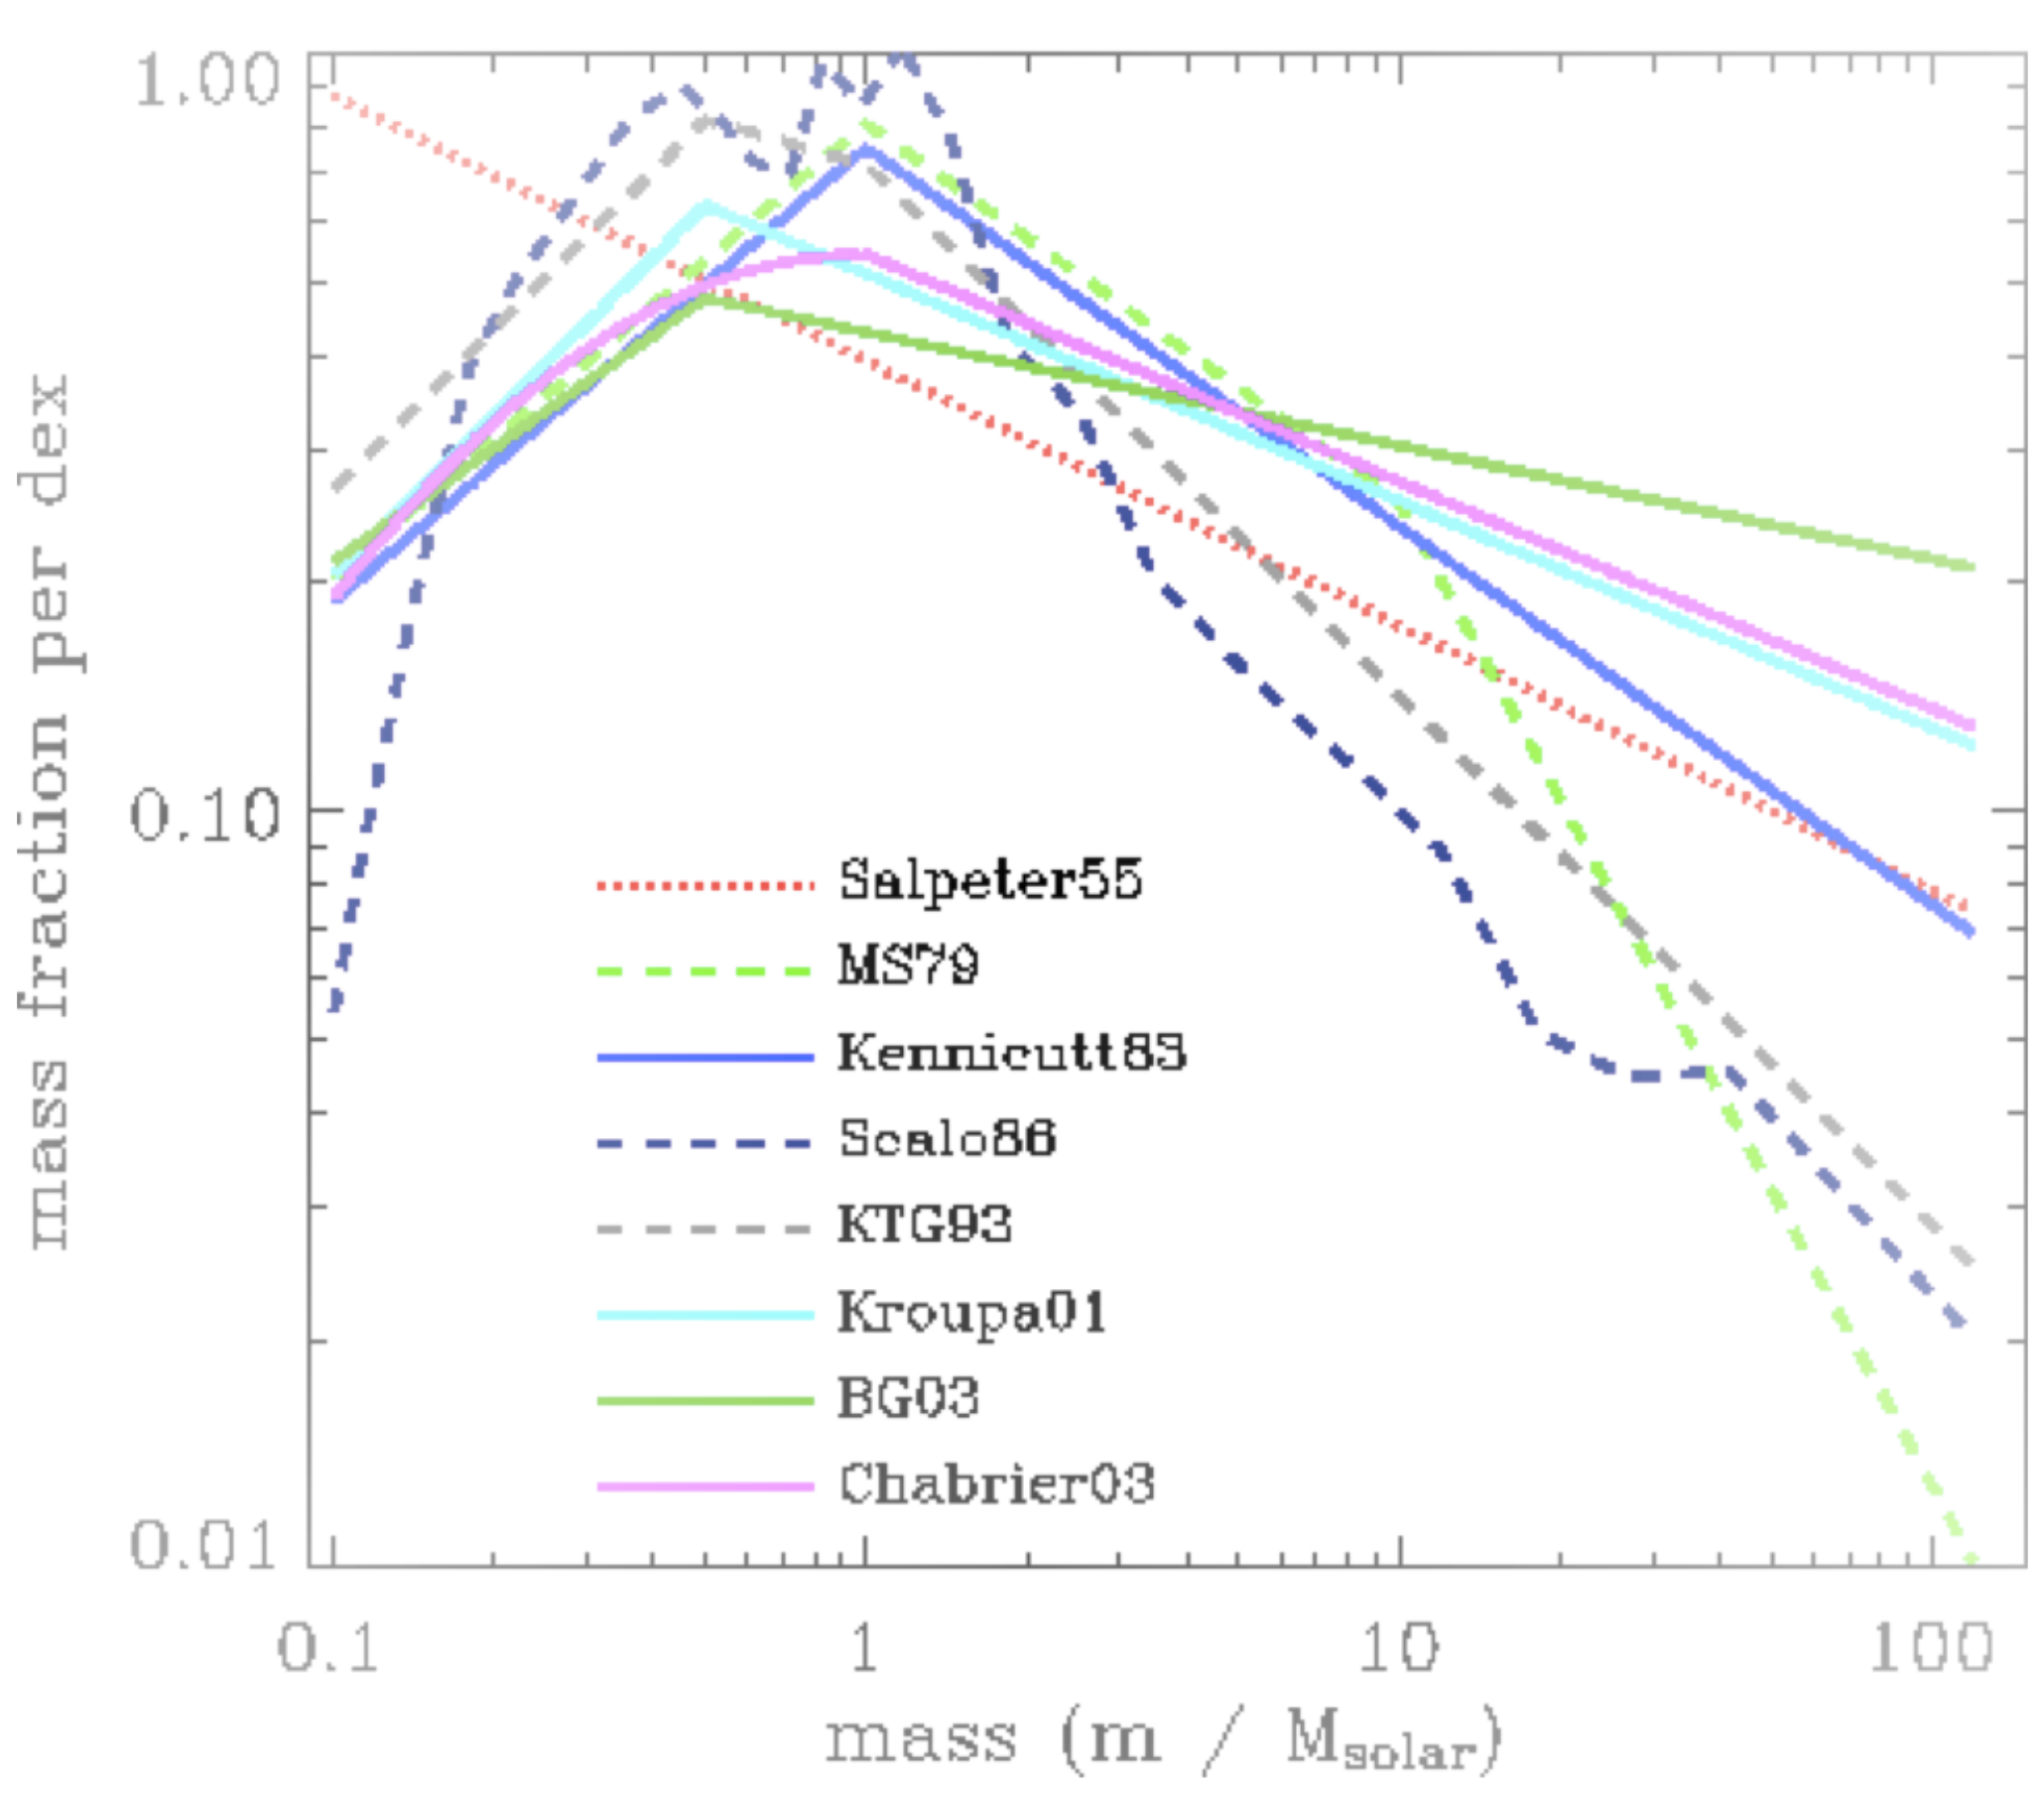
\includegraphics[width=16cm]{../image_intro/imf}
\small
\caption{Comparing stellar initial mass functions (IMFs) by plotting the mass fraction per dex, power of 10, versus mass, normalized so that the integral under each curve is unity. The mass ranges from 0.1 to 120~M$_\odot$. Adopted from~\cite{Baldry03}.} 
\end{figure}


Since in using SFR calibration for different galaxies, we assume the initial mass function is universal, careful measurement of the IMF is the key factor in understanding the star formation rate. 
In distant galaxies, only massive stars can be detected; therefore, the IMF must be assumed to include all stellar mass ranges in the SFR calibrations. 
To show the impact of the different stellar IMF assumptions on the SFR calibrations, \cite{Calzetti13} used two different stellar IMFs and derived the SFR calibrations with these new assumptions.
Adopting a modified \cite{Kroupa01} IMF, with its maximum stellar mass set to 30~M$_{\odot}$ instead of 100~M$_{\odot}$, changes the SFR calibration constants by factors ranging from 1.4 to 5.6 for different SFR indicators (Tab.~\ref{table1}). 

\subsection{SFR Indicators}

One of the main issues in studying star formation in distant galaxies is the calibration of star formation rate indicators~\citep[e.g.,][]{Lee10}. 
Calibration of SFR indicators can be affected by differences in star formation history (SFH), metallicity, distribution of stellar population and dust in galaxies~\citep{Calzetti13}. 
Based on the spatial resolution of a system, one can divide star formation indicators into two categories: resolved and unresolved star formation indicators.

\subsubsection{Resolved Star Formation Indicators}
The most direct way to measure the SFR and trace recent star formation is counting individual objects~\citep{Kennicutt12}. 
These objects mostly few million years old and usually are referred to as young stellar objects (YSOs). 
Counting YSOs is used for calculating star formation rates in molecular clouds within $0.5- 1$ kpc of the Solar System. 
The number of YSOs can be converted to SFR using: 
\begin{equation}
SFR(YSO) = N_{yso} <M>/\tau 
\end{equation}
where SFR(YSO) is in units of M$_{\odot}$~yr$^{-1}$, N$_{yso}$ is the number of YSOs.
$<$M$>$ is the mean mass of YSO which depends on the IMF and considering current IMFs $<$M$> = $0.5~M$_{\odot}$ ~\citep[][]{Kennicutt12}. 
$\tau$ is the lifetime of the YSO  $\tau \sim 2$Myr~\citep{Evans09}. 
Since our current devises cannot resolve individual YSOs, this method can only be applied to the Milky Way and its neighbourhood. 

In theory, for any system with high enough spatial resolution, counting YSOs can be used as a tracer of the star formation. 
However, considering the limited capabilities of the present instruments, YSOs in most regions beyond the Magellanic Clouds (satellite galaxies of the Milky way with distance of 0.05 Mpc) can not be resolved. 
Therefore, most studies use the emission from the energetic young stars as a tracer of the SFR. 

%% to be continued